% Why prediction is important?
\label{sec:prediction}
This section further motivates predictive false sharing and explains how to support it in the runtime system.  

\subsection{Overview}
%\begin{figure*}[!htb]
\label{sec:predictoverview}

\begin{figure}[!t]
\begin{center}
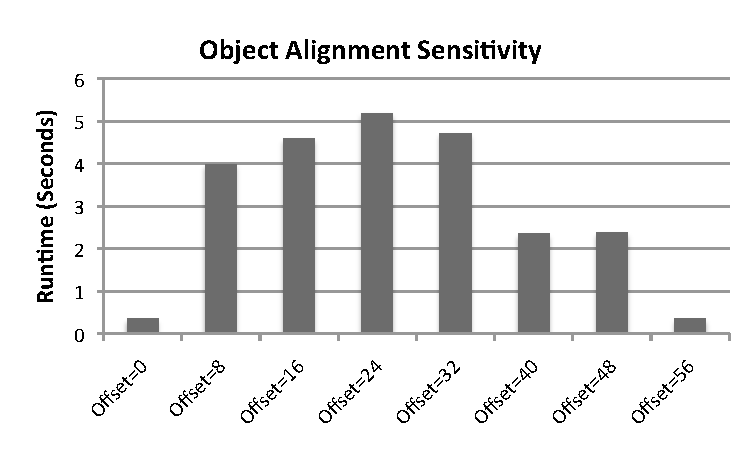
\includegraphics[width=3.3in]{fig/perfsensitive}
\end{center}
\caption{
Performance of the linear\_regression benchmark from the Phoenix benchmark suite.
Performance is highly sensitive to the offset of the starting address of the (potentially) falsely-shared object 
and the start of the cache line. 
\label{fig:perfsensitive}}
\end{figure}

False sharing can depend on 
the alignment of objects and corresponding cache lines.
Figure~\ref{fig:perfsensitive} demonstrates the impact of placement on linear\_regression, a benchmark from the Phoenix benchmark suite.
For this benchmark,
when the offset of the starting address between the potentially falsely-shared object and corresponding cache lines 
is $0$ or $56$ bytes, 
there is no false sharing. 
When the offset is $24$ bytes, we see the most severe performance effect caused 
by false sharing. 
The performance difference between these two scenarios can be as great as $15\times$.
 
Existing detection tools only report observed false sharing.
In this case, they would miss a severe false sharing problem that could occur in the wild if the offset of the starting 
address was $0$ bytes or $56$ bytes in their test environment.
\Predator{} overcomes this shortcoming by accurately predicting potential false sharing.

\begin{figure*}
\begin{center} 
\subfigure[No false sharing]{%
   \label{fig:nofs}
   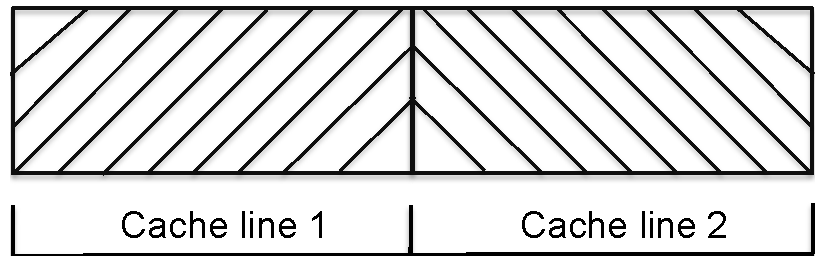
\includegraphics[width=0.24\textwidth]{fig/Potential1}
}%
\hspace{30pt}
\subfigure[False sharing with larger cache size]{%
   \label{fig:fslarger}
   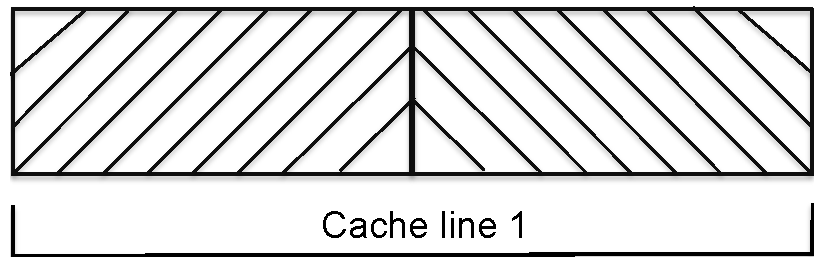
\includegraphics[width=0.24\textwidth]{fig/Potential2}
}%
\hspace{30pt}
\subfigure[False sharing with different alignment]{%
   \label{fig:fsnoalignment}
   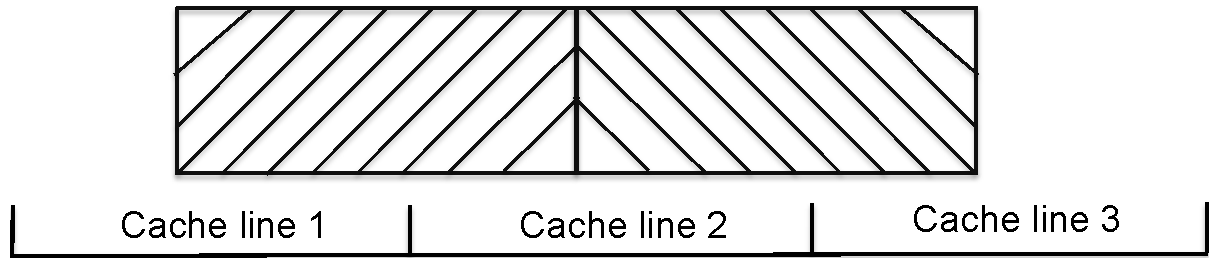
\includegraphics[width=0.36\textwidth]{fig/Potential3}
}%
\end{center}
%\includegraphics{fig/potential.pdf}
\caption{False sharing under different scenarios (see Section~\ref{sec:predictoverview}).}
\label{fig:potentialfalsesharing}
\end{figure*}

\Predator{} predicts {\it potential false sharing}, the type of
false sharing that does not 
manifest in the current execution but may appear and greatly affect programs' performance
in a slightly different environment.

Figure~\ref{fig:potentialfalsesharing} presents a simplified overview of how false sharing can be triggered 
 by different environments.
In this figure, two rectangles with different patterns
represent two portions of the same object, updated by different threads. 
In Figure~\ref{fig:nofs}), there is no false sharing when thread T1 only updates 
cache line 1 and T2 only updates cache line 2.
However, false sharing appears in each of the following cases, even with the same
access pattern:

\begin{itemize}
\item \textbf{Doubling the cache line size.} (Figure~\ref{fig:fslarger}) When the size of a
cache line doubles,
both T1 and T2 access the same cache line, leading to false sharing.

\item \textbf{Different object starting addresses.} (Figure~\ref{fig:fsnoalignment})
If the starting address of the object is not aligned with the starting address of 
the first cache line, 
T1 and T2 can update the second cache line simultaneously, 
causing false sharing. 
\end{itemize} 

\Predator{} predicts whether programs can have potential false sharing  
in either of these two scenarios. These scenarios capture the impact of any change in the execution environment, such as a different hardware platform or a different memory allocation sequence.

\subsection{Basic Prediction Workflow}
\label{sec:predictionmechanism} 

\Predator{} focuses exclusively on potential false sharing that can 
cause performance problems.
Its implementation is based on
two key observations. First, only accesses to 
adjacent cache lines can lead to potential false sharing: 
that is, they introduce cache invalidations when the cache line size
or an object's starting address changes.
Second, only when false sharing introduces a large number of cache invalidations
can it degrade performance.

Based on these two observations, \Predator{} employs 
the following workflow to detect potential false sharing.
Note that the detection optimizations listed in Section~\ref{optimization} apply directly to prediction as well.

\begin{enumerate}
\item
Track the number of writes to different cache lines. 

\item
When the number of writes to a cache line $L$ reaches {\it TrackingThreshold},
track detailed read and write accesses for every word in both cache line $L$ 
and its adjacent cache lines. 

\item
When the number of writes to a cache line $L$ crosses a second threshold (the 
{\it PredictionThreshold}), 
identify whether there exists false sharing in $L$ and its adjacent 
cache lines by analyzing word access information collected in Step 2. 
Section ~\ref{sec:evaluatingfs} describes this process.

\item
If potential false sharing is found, continue to track cache line invalidations to confirm it. Section~\ref{sec:tracking} discusses the details.
 
\end{enumerate}

\subsection{Searching for Potential False Sharing}
\label{sec:evaluatingfs}

To predict potential false sharing in the cases when either the hardware cache line size doubles or when object placement changes, we first 
introduce the concept of a \emph{virtual cache line}.  A virtual cache line
is a contiguous memory range that spans one or more physical cache 
lines.

Using virtual cache lines lets \Predator{} predict potential false sharing in both of the scenarios mentioned above. When the hardware cache line size doubles, a virtual line is
composed of two original contiguous cache lines and the first cache
line has an even index number.  Thus, only cache lines $2*i$ and
$2*i+1$ can form a virtual line.  To predict false sharing due to different starting
addresses, a virtual line can have the same size as physical lines,
but can be positioned arbitrarily: unlike actual cache lines, the
starting address of a virtual cache line does not need to be multiple
of the cache line size.  For instance, a 64-byte long virtual line can
consist of the range $[0,64)$ bytes or $[8,72)$ bytes.

To search for potential false sharing problems, 
\Predator{} searches for a hot access pair on line $L$ and its adjacent cache lines 
by analyzing the detailed word access information collected in Step 2. 
A hot access in a cache line refers to a word whose number of read or write accesses 
is larger than the average number of accesses to each word of cache line $L$.
For every hot access $X$ in cache line $L$, \Predator{} searches for another
hot access $Y$ in $L$'s previous cache line or next cache line satisfying
the following conditions: 
(1) $X$ and $Y$ reside in the same virtual line;
(2) at least one of $X$ or $Y$ are a write access; and 
(3) $X$ and $Y$ are issued by different threads.

 
Whenever it finds such a pair $X$ and $Y$, 
\Predator{} identifies potential performance-degrading false sharing whenever
 the number of cache invalidations caused by $X$ and $Y$, at a possible virtual line, 
is greater than the average number of accesses on each word of $L$. 
This approach is based on a the same observation as in detection:
\emph{if a thread writes a virtual line after other threads 
have accessed the same virtual line, this write operation most likely causes at least one cache 
invalidation}. 
\Predator{} conservatively assumes that accesses from different threads occurs in an interleaved manner; that is, it assumes that the schedule exposes false sharing.
This approach ensures that \Predator{} does not miss any potential false sharing cases.
  
After identifying possible false sharing, \Predator{} goes to Step 4 to 
verify whether this is an actual false sharing problem.

\subsection{Verifying Potential False Sharing}
\label{sec:tracking}

\Predator{} verifies potential false sharing by tracking 
cache invalidations of a problematic virtual line.

For potential false sharing caused by double cache line size, as described in
Section~\ref{sec:evaluatingfs}, a virtual line is always composed of 
cache line with index $2*i$ and $2*i+1$. 
\Predator{} tracks cache invalidations
on the virtual line on which false sharing has been discovered.

However, for the case of a change in starting address,
two hot accesses with a distance less than the cache line size 
can form multiple virtual lines. 
There is thus an additional step required to determine which virtual line needs to be tracked.
%\Predator{} utilizes the virtual line to simulate the effect of changing the 
%starting addresses of objects.


\begin{figure}
\begin{center} 
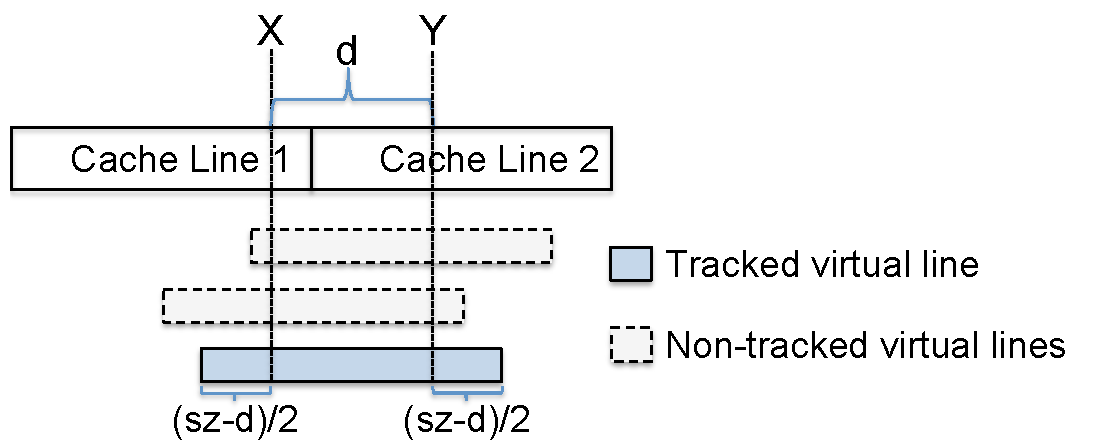
\includegraphics[width=3.3in]{fig/trackpotential}
\end{center}
\caption{Determining a virtual line with size $sz$ according to hot accesses (see Section~\ref{sec:tracking}).
\label{fig:trackpotential}}
\end{figure}

Given two words with the hot accesses shown in Figure~\ref{fig:trackpotential}, 
\Predator{} leaves the same space before $X$ and after $Y$ in determining a virtual line. 
That is, the virtual line starting 
at location $X-((sz-d)/2)$ and ending at $Y+((sz-d)/2)$ is tracked. 
This choice allows tracking more possible cache invalidations caused by
adjacent accesses to $X$ and $Y$. 
Since adjusting the starting address of a virtual line has the same effect as
adjusting the starting address of an object in detecting false sharing,
all cache lines related to the same object must be adjusted at the same time.
\Predator{} then tracks cache invalidations based on these adjusted virtual lines.


